%%%%%%%%%%%%%%%%%%%%%%%%%%%%%%%%%%%%%%%%%
% Professional Mathematical Presentation Template
% 
% This template uses the beamer class with the Madrid theme
% and a custom color scheme for a clean, professional look
% that works well with mathematical content.
%%%%%%%%%%%%%%%%%%%%%%%%%%%%%%%%%%%%%%%%%
\documentclass[aspectratio=169]{beamer} % 16:9 aspect ratio (modern)
% Theme settings
\usetheme{Madrid}
\usecolortheme{default}
\usepackage[dvipsnames]{xcolor}
\definecolor{primcolor}{RGB}{25,50,100} % Dark blue
\setbeamercolor{structure}{fg=primcolor}
\setbeamercolor{frametitle}{bg=primcolor!15, fg=primcolor}
\setbeamercolor{title}{fg=white} % White title text for contrast
\setbeamercolor{subtitle}{fg=white} % White subtitle text
\setbeamercolor{author}{fg=primcolor} % White author text
\setbeamercolor{date}{fg=primcolor} % White date text
\setbeamercolor{institute}{fg=primcolor} % White institute text
% Font settings
\usefonttheme{professionalfonts}
\usefonttheme{serif}
% Package imports
\usepackage{amsmath, amsfonts, amssymb, amsthm} % Math packages
\usepackage{mathtools} % Enhanced math tools
\usepackage{bm} % Bold math symbols
\usepackage{graphicx} % For images
\usepackage{booktabs} % Professional tables
\usepackage{tikz} % For diagrams
\usetikzlibrary{arrows, positioning, matrix, decorations.pathreplacing}
% Use beamer's theorem styles
\setbeamertemplate{theorem}[ams style]
\setbeamertemplate{theorems}[numbered]
% Remove navigation symbols
\setbeamertemplate{navigation symbols}{}
% Custom footer
\setbeamertemplate{footline}{
  \leavevmode%
  \hbox{%
  \begin{beamercolorbox}[wd=.333333\paperwidth,ht=2.25ex,dp=1ex,center]{author in head/foot}%
    \usebeamerfont{author in head/foot}\insertshortauthor
  \end{beamercolorbox}%
  \begin{beamercolorbox}[wd=.333333\paperwidth,ht=2.25ex,dp=1ex,center]{title in head/foot}%
    \usebeamerfont{title in head/foot}\insertshorttitle
  \end{beamercolorbox}%
  \begin{beamercolorbox}[wd=.333333\paperwidth,ht=2.25ex,dp=1ex,right]{date in head/foot}%
    \usebeamerfont{date in head/foot}\insertshortdate{}\hspace{2em}
    \insertframenumber{} / \inserttotalframenumber\hspace{2ex} 
  \end{beamercolorbox}}%
  \vskip0pt%
}
% Title information
\title[GNN]{How Powerful Are Graph Neural Networks?}
\subtitle{Xu et al 2021}
\author[Longye]{Longye Tian \\ \texttt{longye.tian@anu.edu.au}}
\institute[ANU]{Australian National University\\ School of Economics}
\date{May 12th, 2025}
\DeclareFontFamily{U}{mathx}{\hyphenchar\font45}
\DeclareFontShape{U}{mathx}{m}{n}{
      <5> <6> <7> <8> <9> <10>
      <10.95> <12> <14.4> <17.28> <20.74> <24.88>
      mathx10
      }{}
\DeclareSymbolFont{mathx}{U}{mathx}{m}{n}
\DeclareMathSymbol{\bigtimes}{1}{mathx}{"91}

\begin{document}

% Title frame
\begin{frame}
  \titlepage
\end{frame}

% Outline frame
\begin{frame}{Big Picture}
    \begin{itemize}
        \item What Graph Neural Net(GNN) can do and cannot do?
        \item Empirical success but limited theoretical research
        \item How expressive are different GNN architectures in capturing and distinguishing graph structures?
    \end{itemize}
\end{frame}

\begin{frame}{Motivation - US and Australian economy}
\begin{figure}
    \centering
    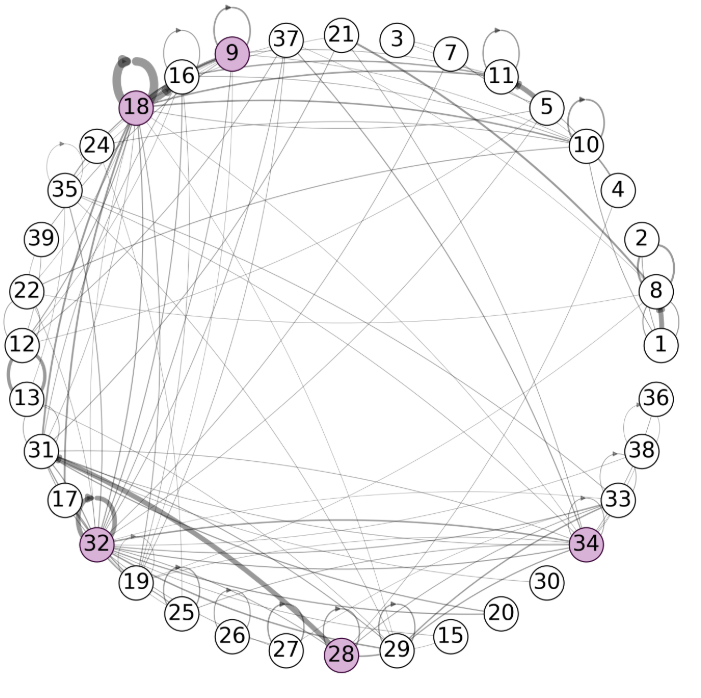
\includegraphics[width=0.5\linewidth]{Network/Graph Neural Network/au-net.png}
    \caption{Australian Production network}
\end{figure}
\end{frame}

\begin{frame}{Motivation - US and Australian economy}
\begin{figure}
    \centering
    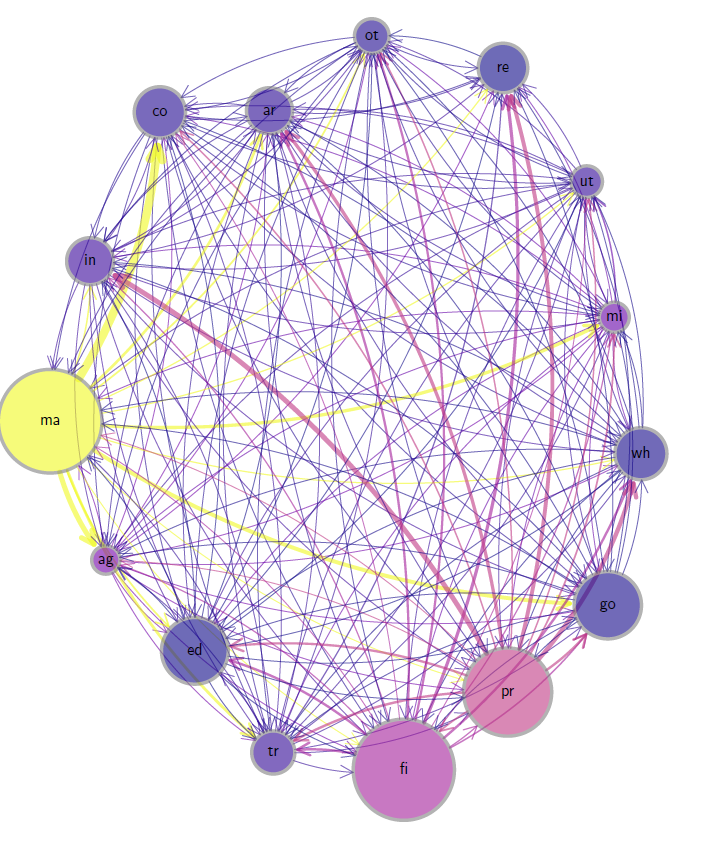
\includegraphics[width=0.4\linewidth]{Network/Graph Neural Network/us-net.png}

\end{figure}
    
\end{frame}
\begin{frame}{Weisfeilei-Lehman (WL) test}
\begin{figure}
    \centering
    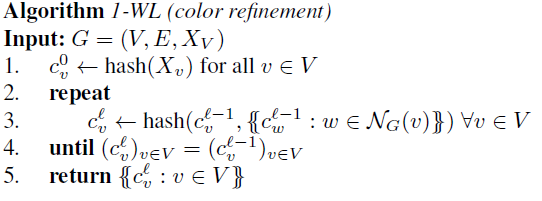
\includegraphics[width=0.8\linewidth]{Network/Graph Neural Network/Weisfeiler-Lehman.png}
\end{figure}
\end{frame}
\begin{frame}{What is GNN? Setup}
\begin{itemize}
    \item $G = (V,E, X_V)$    
    \item In the $k$-th layer
    $$
    h_v^{k} = COMBINE^{(k)}\left(h_v^{k-1}, a_v^{(k)}\right), a_v^{(k)} = AGGREGATE^{(k)}\left(\{h_u^{k-1}: u\in \mathcal{N}(v)\}\right\)
    $$
    \item Looks really like the iteration step in the WL test
\end{itemize} 
\end{frame}
\begin{frame}{Key Theorem}
    \begin{theorem}
        No message-passing GNN can be more powerful than the 1-WL test at distinguishing graph structure.
    \end{theorem}
    \begin{theorem}
        GNN can achieve this theoretical upper bound using the GIN architecture
    \end{theorem}
    What is GIN?
\end{frame}
\begin{frame}{Graph Isomorphic Network}
GIN:
$$
h^{(k)}_v = MLP\left(\underbrace{(1+\epsilon)h^{(k-1)}_v}_{\text{center node}}+\underbrace{\sum_{u\in N(v)} h^{(k-1)}_u}_{\text{neighbors}}\right)
$$
\begin{itemize}
    \item The sum aggregator preserves multiset cardinality
    \item MLP(NN) has the universal approximation properties
    \item As powerful as 1-WL test
\end{itemize}
\end{frame}
\begin{frame}{Discussion}
\begin{itemize}
    \item Is 1-WL good enough? (Fail to distinguish regular graph with $n$ nodes)
    \begin{figure}
        \centering
        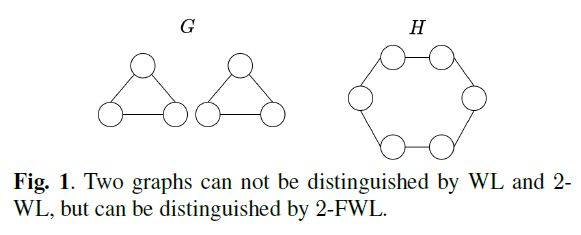
\includegraphics[width=0.7\linewidth]{Network/Graph Neural Network/1-WL fail.png}
    \end{figure}
    \item Difficulty lies at the tradeoff: Computational complexity and expressiveness 
\end{itemize}
    
\end{frame}
\begin{frame}{Future outlooks}
\begin{itemize}
\end{itemize}
    
\end{frame}
\end{document}
